\documentclass{article}

\usepackage[margin=0.5in]{geometry}
\usepackage{multicol}
\usepackage{tikz}
\usepackage{amsthm}
\usepackage{amsmath}

\theoremstyle{definition}
\newtheorem*{solution}{Solution}

\title{Triangles Set B}
\date{}
\author{}

\begin{document}
\maketitle

\begin{multicols}{2}
    \begin{enumerate}
        \item An ant is crawling along the outside of the box.
            What is the shortest distance he can walk from $A$ to $B$ along the path shown?
            \begin{center}
                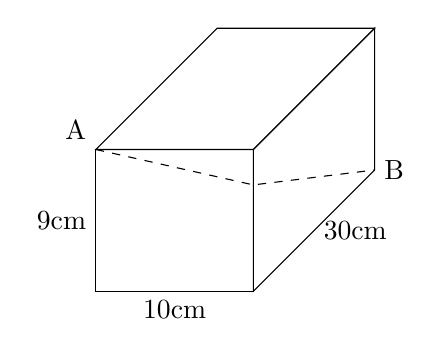
\begin{tikzpicture}
                    \coordinate[label=above left:A] (A) at (0,1.8,4);
                    \coordinate[label=right:B] (B) at (2,0,0);
                    \draw (0,0,4) -- node[left] {9cm} (0,1.8,4) -- (A) -- (2,1.8,4) -- (2,0,4) -- node[below] {10cm} (0,0,4) -- cycle;
                    \draw (B) -- node[right] {30cm} (2,0,4) -- (2,0,4) -- (2,1.8,4) -- (2,1.8,0) -- cycle;
                    \draw (0,1.8,0) -- (2,1.8,0) -- (2, 1.8, 4) -- (A) -- cycle;
                    \draw[dashed] (A) -- (2,1.35,4) -- (B);
                \end{tikzpicture}
            \end{center}
            \begin{solution}
                Unfold the left side of the box to see that we are solving for the diagonal length of a $9$ by $40$ rectangle.
                The Pythagorean theorem gives us $41$.
            \end{solution}
        \item There is a shorter path from $A$ to $B$ in the diagram above.
            What is the shortest distance along the outside of the box from $A$ to $B$?
            Express your answer as a decimal rounded to the nearest tenth.
            \begin{solution}
                We look to ``unfold'' the box in a way that will give us the rectangle with the shortest diagonal.
                There are three ways in this case.
                Problem $1$ gave us a $9$ by $40$ rectangle, using the top and right sides gives us a $10$ by $39$ rectangle, and using the top and the front gives us a $19$ by $30$ rectangle.
                To minimize the diagonal, we look for the rectangle whose sides are closest in length.
                The shortest distance is the diagonal of a $19$ cm by $30$ cm rectangle, which is approximately $35.5$ by the Pythagorean theorem.
            \end{solution}
        \item An equilateral triangle is stacked above a square as shown, with a circle inscribed inside the square and two stacked circles inscribed in the triangles so that they are tangent to each other.
            What is the ratio of the area of the smallest circle to the area of the largest circle?
            Express your answer as a common fraction.
            \begin{center}
                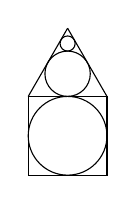
\begin{tikzpicture}
                    \draw (0,0) -- (1,0) -- (1,1) -- (0,1) -- cycle;
                    \draw (0.5,0.5) circle (0.5cm);
                    \draw (0,1) -- ++(60:1);
                    \draw (1,1) -- ++(120:1);
                    \draw (0.5, 1.288) circle (0.288);
                    \draw (0.5, 1.672) circle (0.096);
                \end{tikzpicture}
            \end{center}
            \begin{solution}
                Let's assume the square has side length $2$.
                Then the largest circle has a radius of $1$ and its area is $\pi \cdot 1^2 = \pi$.
                If we draw a line from the top vertex of the equilateral triangle to the midpoint of the bottom edge, we divide the triangle into two $30$-$60$-$90$ triangles.
                The short leg of one of these triangles has length $1$, so the long leg has length $\sqrt{3}$.
                This is also the height of the equilateral triangle.
                If we draw lines from the center of the medium circle to the two bottom vertices of the triangle, we form a smaller triangle which shares a base with the equilateral triangle.
                This triangle's area is clearly $\frac{1}{3}$ of the area of the equilateral triangle, and since the area of a triangle is proportional to its height, the height of this smaller triangle which is also the radius of the medium circle is $\frac{1}{3}$ the height of the equilateral triangle.
                So the radius of the medium circle is $\frac{\sqrt{3}}{3}$.
                If we draw a horizontal line passing in between the medium and the small circle, we form a smaller equilateral triangle at the top.
                Subtracting the diameter of the medium circle from the height of the larger equilateral triangle, we obtain the height of the smaller equilateral triangle, which is $\frac{\sqrt{3}}{3}$.
                We have established that the radius of a circle inscribed in an equilateral triangle is $\frac{1}{3}$ the height of the equilateral triangle, so the radius of the small circle is $\frac{\sqrt{3}}{9}$.
                This means it's area is $\frac{\pi}{27}$, so the ratio between the area of the small circle and the area of the large circle is $\frac{1}{27}$.
            \end{solution}
        \item What is the height of a STOP sign (regular octagon) whose sides are one foot long?
            \begin{solution}
                If we extend the sides of two pairs of opposite edges so that we create a square surrounding the octagon, there would be four $45$-$45$-$90$ triangles with a hypotenuse of $1$ at each corner.
                This makes one of their legs $\frac{\sqrt{2}}{2}$.
                The height of the octagon is the length of one edge plus the length of two legs of the corner triangles, or $1 + 2 \cdot \frac{\sqrt{2}}{2} = 1 + \sqrt{2}$.
            \end{solution}
        \item Three circles, each having a radius of $4$ units, are externally tangent to each other.
            A triangle joins the centers of the circles.
            What is the area of the shaded region within the triangle but outside the circles?
            Express your answer as a decimal to the nearest tenth.
            \begin{center}
                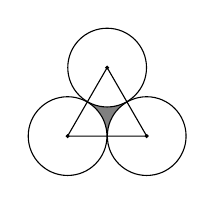
\begin{tikzpicture}
                    \draw[fill=gray] (90:0.58) -- (210:0.58) -- (330:0.58) -- cycle;
                    \foreach \angle in {90, 210, 330}
                    {
                        \begin{scope}
                            \clip (\angle:0.58) circle (0.5cm);
                            \fill[white] (\angle:0.58) circle (0.5cm);
                        \end{scope}
                        \draw (\angle:0.58) circle (0.5cm);
                        \filldraw (\angle:0.58) circle (0.5pt);
                    }
                    \draw (90:0.58) -- (210:0.58) -- (330:0.58) -- cycle;
                \end{tikzpicture}
            \end{center}
            \begin{solution}
                At each vertex of the triangle, the sector of the circle is $\frac{1}{6}$ of a full circle.
                The three sectors have a combined area equivalent to $\frac{3}{6} = \frac{1}{2}$ of a circle with a radius of $4$ units.
                That area is $\frac{1}{2} \pi r^2 = \frac{1}{2} \pi \cdot 4^2 = 8\pi$ units$^2$.
                The triangle has side length equal to twice the radius of a circle, or $8$ units, and its altitude is $4\sqrt{3}$ units
                Thus the triangle has area $\frac{1}{2} bh = \frac{1}{2} \cdot 8 \cdot 4\sqrt{3} = 16\sqrt{3}$ units$^2$.
                The shaded region within the triangle but outside the circles has area $16\sqrt{3} - 8\pi \approx 2.6$ units$^2$.
            \end{solution}
    \end{enumerate}
\end{multicols}
\end{document}
